\section{Requisiti}\label{Requisiti}

I requisiti vengono classificati ed assegnati con un identificativo univoco, secondo quanto definito nel documento \textit{Norme di progetto v2.0.0.}
\\
Di seguito, viene riportato il contenuto della classificazione dei requisiti per facilitare i lettori esterni che non hanno accesso al documento.
\\
Ogni requisito, nel documento, deve seguire le seguenti regole di identificazione:
\begin{center}
	\textbf{R[Importanza][Tipo][Identificativo]}
\end{center}  
\begin{itemize}
	\item \textbf{R}: sta per appunto "requisito";
	\item \textbf{Importanza}: specifica quanto è importante il requisito, può assumere tre valori:
	\begin{itemize}
		\item \textbf{O}: indica che il requisito è obbligatorio, e deve essere per forza soddisfatto per il corretto funzionamento di base del sistema;
		\item \textbf{D}: indica che il requisito è desiderabile, se viene soddisfatto aumenta la completezza del sistema, se non viene soddisfatto non crea alcuna penalizzazione;
		\item \textbf{F}: indica un requisito opzionale (F sta per "facoltativo"). 
	\end{itemize}
	\item \textbf{Tipo}: specifica la tipologia e può assumere i seguenti valori:
	\begin{itemize}
		\item \textbf{F}: requisito funzionale;
		\item \textbf{P}: requisito prestazionale;
		\item \textbf{Q}: requisito qualitativo;
		\item \textbf{V}: requisito di vincolo.
	\end{itemize}
	\item \textbf{Identificativo}: numero progressivo che identifica il requisito, strutturato come segue: 
	\begin{center}
		\textbf{[codice padre].[codice figlio]}	
	\end{center}
\end{itemize}

\newpage
\subsection{Requisiti Funzionali}\label{RF}
\begin{center}
\begin{longtable}[c]{|m{.13\textwidth}|m{.47\textwidth}|m{.2\textwidth}|m{.11\textwidth}|}
\hline
\rowcolor{bluelogo}\textbf{\textcolor{white}{ID}} & \textbf{\textcolor{white}{Descrizione}} & \textbf{\textcolor{white}{Obbligatorietà}} & \textbf{\textcolor{white}{Fonti}}\\
\hline \hline
\endhead
ROF1 & L'utente deve poter aggiungere una rete bayesiana al sistema & Obbligatorio & UC1\\
\hline
\rowcolor{grigio}ROF1.1 & Il Sistema deve mettere a disposizione un pulsante per avviare l'operazione di selezione del file, contente la definizione della rete, da caricare & Obbligatorio & UC1\\
\hline
ROF1.2 & Il Sistema deve consentire all'utente di selezionare un file da caricare & Obbligatorio & UC1\\
\hline
\rowcolor{grigio}ROF1.3 & Il Sistema deve mettere a disposizione dell'utente un bottone per avviare l'operazione di caricamento & Obbligatorio & UC1\\
\hline
ROF1.4 & Il Sistema deve visualizzare un messaggio di errore nel caso l'operazione di caricamento del file non sia andata a buon fine & Obbligatorio & UC1 UC8\\
\hline
\rowcolor{grigio}ROF1.4.1 & Il Sistema deve controllare l'estensione del file caricato, accettando come input solamente file in formato \textit{JSON} & Opzionale & UC1 UC8\\
\hline
RFF1.4.2 & Il Sistema deve visualizzare un messaggio di errore nel caso in cui la struttura interna del file selezionato sia errata & Opzionale & UC1 UC8\\
\hline
\rowcolor{grigio}ROF1.5 & Il Sistema deve interpretare il file caricato, al fine di costruire la rete bayesiana attraverso la sua definizione & Obbligatorio & UC1\\
\hline
RDF1.6 & Il Sistema deve mantere in memoria, in caso di riavvio, l'ultima rete bayesiana caricata dall'utente & Desiderabile & Decisione Interna\\
\hline
\rowcolor{grigio}ROF2 & L'utente deve poter collegare un flusso di dati ad ogni nodo desiderato della rete preesistente & Obbligatorio & UC2\\
\hline
ROF2.1 & Il Sistema deve interpretare la rete bayesiana caricata, al fine di estrapolarne i nodi e fornirli all'utente sotto forma di lista & Obbligatorio & UC2\\
\hline
\rowcolor{grigio}ROF2.1.1 & Il Sistema deve mostrare, per ogni nodo, il nominativo dello stesso & Obbligatorio & UC2\\
\hline
ROF2.1.2 & Il Sistema deve mostrare, per ogni nodo, una corrispondente checkbox che identifichi lo stato dello stesso: collegato ad un flusso dati oppure no & Obbligatorio & UC2\\
\hline
\rowcolor{grigio}ROF2.5 & Il Sistema deve mettere a disposizione dell'utente le impostazioni necessarie per effettuare correttamente il collegamento desiderato & Obbligatorio & UC2\\
\hline
ROF2.5.1 & Il Sistema, in seguito al click dell'utente su un nominativo, deve aprire una finestra contente un elenco delle sorgenti di dati disponibili per il collegamento & Obbligatorio & UC2.2\\
\hline
\rowcolor{grigio}ROF2.5.2 & L'utente deve poter selezionare la sorgente dati desiderata per il collegamento & Obbligatorio & UC2.2\\
\hline
ROF2.5.3 & Il Sistema deve fornire un elenco dei flussi dati disponibili contestualmente alla sorgente di dati selezionata & Obbligatorio & UC2.2\\
\hline
\rowcolor{grigio}ROF2.5.4 & L'utente deve poter selezionare il flusso dati desiderato per il collegamento & Obbligatorio & UC2.2\\
\hline
ROF2.5.5 & Il Sistema deve mostrare la lista dei possibili stati del nodo selezionato & Obbligatorio & UC2.2\\
\hline
\rowcolor{grigio}ROF2.5.6 & Il Sistema deve mettere a disposizione dell'utente, per ogni stato del nodo, i campi dati necessari alla definizione di un livello di soglia connesso al flusso dati selezionato & Obbligatorio & UC2.2\\
\hline
ROF2.5.6.1 & Il Sistema deve mettere a dispozione dell'utente un campo dati che permetta di definire il valore numerico della soglia & Obbligatorio & UC2.2\\
\hline
\rowcolor{grigio}ROF2.5.6.2 & Il Sistema deve mettere a dispozione dell'utente un campo dati che permetta di definire se il valore numerico definito per la soglia sia un minimo oppure un massimo & Obbligatorio & UC2.2\\
\hline
RDF2.5.6.3 & Il Sistema deve mettere a dispozione dell'utente un campo dati che permetta di definire se la soglia sia critica oppure no & Desiderabile & UC2.2 VER-2019-02-08\\
\hline
\rowcolor{grigio}ROF2.5.7 & L'utente deve poter editare i campi dati per definire correttamente un livello di soglia al di sotto, o al di sopra del quale la probabilità associata a quel dato stato risulta pari al 100\%, mentre le probabilità associate agli altri stati risultano pari allo 0\% & Obbligatorio & UC2.2\\
\hline
ROF2.5.8 & Il Sistema deve mettere a disposizione dell'utente un bottone per confermare le scelte riguardardanti la definizione della soglia & Obbligatorio & UC2.2\\
\hline
\rowcolor{grigio}ROF2.5.9 & Il Sistema deve visualizzare un messaggio di errore nel caso in cui l'utente abbia confermato le proprie scelte riguardanti il collegamento del singolo nodo in esame senza aver correttamente definito il livello di soglia & Obbligatorio & UC2.2 UC14\\
\hline
ROF2.5.10 & Il Sistema deve aggiornare la lista di checkbox, registrando il nuovo stato di ogni nodo (collegato o meno ad un flusso dati) & Obbligatorio & UC2\\
\hline
\rowcolor{grigio}ROF2.6 & Il Sistema deve mettere a disposizione dell'utente un bottone per confermare il collegamento dei nodi & Obbligatorio & UC2\\
\hline
ROF2.7 & Il Sistema deve visualizzare un messaggio di errore nel caso in cui l'utente abbia confermato il collegamento dei nodi senza averne effettivamente collegato alcuno & Obbligatorio & UC2 UC9\\
\hline
\rowcolor{grigio}ROF2.8 & L'utente deve poter modificare il collegamento dei nodi dopo aver confermato le proprie scelte & Obbligatorio & UC2 UC13\\
\hline
ROF2.8.1 & Il Sistema deve rendere non interagibile il pannello contente la lista dei nodi una volta che l'utente abbia effettuato la conferma del collegamento & Obbligatorio & UC2 UC13\\
\hline
\rowcolor{grigio}ROF2.8.2 & Il Sistema deve mettere a disposizione dell'utente un bottone per accedere alla modifica del collegamento dei nodi, rendendo nuovamente interagibile il pannello contente la lista di nodi & Obbligatorio & UC13\\
\hline
ROF2.8.3 & Il Sistema deve interrompere la visualizzazione dei dati ed eliminare eventuali alert ad essi associati nel caso in cui l'utente interagisca con il sistema per modificare il collegamento dei nodi & Obbligatorio & UC2 UC4 UC7 UC13\\
\hline
\rowcolor{grigio}ROF3 & L'utente deve poter impostare una politica temporale per il ricalcolo delle probabilità condizionate associate ai nodi della rete bayesiana & Obbligatorio & UC3\\
\hline
ROF3.3 & L'utente deve avere la possibilità di definire una politica temporale & Obbligatorio & UC3\\ 
\hline
\rowcolor{grigio}ROF3.3.1 & Il Sistema deve mettere a disposizione un pulsante per accedere al pannello di configurazione di una politica temporale & Obbligatorio & UC3\\
\hline
ROF3.3.2 & Il Sistema deve mettere a disposizione dell'utente un pannello di configurazione contente i campi dati necessari alla definizione di una politica temporale & Obbligatorio & UC3.2\\
\hline
\rowcolor{grigio}ROF3.3.2.1 & Il Sistema deve mettere a dispozione dell'utente un campo dati che permetta di definire il valore numerico del timeout ciclico & Obbligatorio & UC3.2\\
\hline
ROF3.3.2.2 & Il Sistema deve mettere a dispozione dell'utente un campo dati che permetta di definire l'unità di misura temporale associata al timeout & Obbligatorio & UC3.2\\
\hline
\rowcolor{grigio}ROF3.3.3 & L'utente deve poter editare i campi dati per definire correttamente la politica temporale desiderata & Obbligatorio & UC3.2\\
\hline
ROF3.4 & Il Sistema deve mettere a disposizione dell'utente un bottone per confermare la politica temporale da lui definita & Obbligatorio & UC3\\
\hline
\rowcolor{grigio}ROF3.5 & Il Sistema deve visualizzare un messaggio di errore nel caso in cui l'utente abbia confermato una politica temporale non correttamente definita & Obbligatorio & UC3 UC15\\
\hline
ROF4 & Il Sistema deve fornire i dati relativi ai nodi della rete bayesiana non collegati al flusso & Obbligatorio & UC4\\
\hline
\rowcolor{grigio}ROF4.4 & Il Sistema deve mettere a disposizione dell'utente un pulsante per avviare il monitoraggio dei dati & Obbligatorio & UC4\\
\hline
ROF4.4.1 & Il Sistema deve visualizzare un messaggio di errore nel caso in cui l'utente abbia avviato il monitoraggio senza aver preventivamente caricato una rete bayesiana & Obbligatorio & UC4 UC10\\
\hline
\rowcolor{grigio}ROF4.4.2 & Il Sistema deve visualizzare un messaggio di errore nel caso in cui l'utente abbia avviato il monitoraggio senza aver preventivamente collegato alcuni dei nodi della rete ad un flusso dati & Obbligatorio & UC4 UC11\\
\hline
ROF4.4.3 & Il Sistema deve visualizzare un messaggio di errore nel caso in cui l'utente abbia avviato il monitoraggio senza aver preventivamente impostato la politica temporale per il ricalcolo delle probabilità & Obbligatorio & UC4 UC12\\
\hline
\rowcolor{grigio}ROF4.5 & Il Sistema deve fornire all'utente una lista di probabilità dinamiche associate ai nodi della rete & Obbligatorio & UC4\\
\hline
ROF4.6 & Il Sistema deve aggiornare periodicamente le probabilità in base a quanto definito come policy per il ricalcolo delle probabilità & Obbligatorio & UC4\\
\hline
\rowcolor{grigio}RDF4.6.1 & Il Sistema, indipendentemente dalla politica temporale stabilita dall'utente, deve ricalcolare le probabilità al verificarsi del superamento di una soglia critica associata ad uno stato di un nodo collegato al flusso di monitoraggio & Desiderabile & UC4 VER-2019-02-08\\
\hline
RFF5 & L'utente deve poter definire alert basati sui dati relativi ai nodi della rete bayesiana non collegati al flusso & Opzionale & UC5\\
\hline
\rowcolor{grigio}RFF5.1 & Il Sistema deve mettere a disposizione di \textit{Grafana} i dati per l'operazione di creazione di alert ad essi associati da parte dell'utente & Opzionale & UC5\\
\hline
RFF5.1.1 & Il pannello "G\&B" deve supportare la funzione di "edit" da parte dell'utente & Opzionale & UC5\\
\hline
\rowcolor{grigio}RFF5.1.2 & Il Sistema deve mettere a disposizione dell'utente un pulsante "Aggiungi Alert" che conduca l'utente alle impostazioni di edit del pannello "G\&B" alla voce "Alert" & Opzionale & UC5\\
\hline
RFF6 & L'utente deve poter visualizzare gli alert creati sulla base dei dati relativi ai nodi della rete bayesiana non collegati al flusso & Opzionale & UC7\\ 
\hline
\rowcolor{grigio}RFF6.1 & Il Sistema deve mettere periodicamente a disposizione della piattaforma \textit{Grafana} i dati aggiornati per il monitoraggio costante dello stato degli alert & Opzionale & UC7\\
\hline
RFF6.2 & L'utente deve poter rimuovere gli alert associati ai nodi della rete bayesiana & Opzionale & UC6\\
\hline
\rowcolor{grigio}RFF6.2.1 & L'utente deve poter selezionare l'alert da eliminare attraverso il pannello di visualizzazione degli alert & Opzionale & UC6\\
\hline
\caption{Requisiti Funzionali}
\end{longtable}
\end{center}


%\subsection{Requisiti Prestazionali}\label{RP}

\subsection{Requisiti di Qualità}\label{RQ}
\begin{center}
\begin{longtable}[c]{|m{.09\textwidth}|m{.48\textwidth}|m{.2\textwidth}|m{.12\textwidth}|}
\hline
\rowcolor{bluelogo}\textbf{\textcolor{white}{ID}} & \textbf{\textcolor{white}{Descrizione}} & \textbf{\textcolor{white}{Obbligatorietà}} & \textbf{\textcolor{white}{Fonti}}\\
\hline \hline
\endhead
ROQ1 & E' necessario fornire un manuale utente, per l'utilizzo del prodotto, in formato \textit{pdf} & Obbligatorio & Capitolato\\
\hline
\rowcolor{grigio}ROQ1.1 & Il manuale utente deve essere disponibile in lingua italiana & Obbligatorio & Decisione Interna\\
\hline
RDQ1.2 & Il manuale utente deve essere disponibile in lingua inglese & Desiderabile & Decisione Interna\\
\hline
\rowcolor{grigio}ROQ2 & E' necessario fornire un manuale per la manutenzione ed estensione del prodotto & Obbligatorio & Capitolato\\
\hline
ROQ2.1 & Il manuale di manutenzione/estensione deve essere disponibile in lingua italiana & Obbligatorio & Decisione Interna\\
\hline
\rowcolor{grigio}RDQ2.2 & Il manuale di manutenzione/estensione deve essere disponibile in lingua inglese & Desiderabile & Decisione Interna\\
\hline
ROQ3 & Il prodotto deve essere sviluppato in modo concorde a quanto stabilito nelle \textit{Norme di Progetto v1.0.0} & Obbligatorio & Decisione Interna\\
\hline
\rowcolor{grigio}RDQ5 & Il codice sorgente del plug-in deve essere reperibile in una repository pubblica su GitHub\glossario o su altre piattaforme di condivisione & Desiderabile & Capitolato \\
\hline
RDQ6 & Il plug-in deve essere pubblicato nella sezione plug-in di \textit{Grafana}, disponibile all'indirizzo \url{https://grafana.com/plugins}   & Desiderabile & Decisione Interna \\
\hline
\caption{Requisiti di Qualità}
\end{longtable}
\end{center}



\subsection{Requisiti di Vincolo}\label{RV}
\begin{center}
\begin{longtable}[c]{|m{.1\textwidth}|m{.53\textwidth}|m{.25\textwidth}|}
\hline
\rowcolor{bluelogo}\textbf{\textcolor{white}{ID}} & \textbf{\textcolor{white}{Descrizione}} & \textbf{\textcolor{white}{Fonti}}\\
\hline \hline
\endhead
ROV1 & Il plug-in deve essere sviluppato in linguaggio \textit{ECMAScript6} & \textit{Grafana}: guida per gli sviluppatori.\\
\hline
\rowcolor{grigio}ROV2 & Il punto di ingresso per il plug-in deve essere sviluppato nel file "module.js" & \textit{Grafana}: guida per gli sviluppatori\\
\hline
ROV3 & Va utilizzato un qualsiasi build system\glossario che supporti \textit{systemjs}\glossario & \textit{Grafana}: guida per gli sviluppatori\\
\hline
\rowcolor{grigio}ROV4 & Il codice sorgente del plug-in deve essere open source & Capitolato\\
\hline
ROV5 & La rete bayesiana è definita in un file formato JSON & Capitolato\\
\hline
\rowcolor{grigio}ROV6 & L'interfaccia grafica del plug-in è sviluppata utilizzando HTML5\glossario e CSS\glossario & \textit{Grafana}: guida per gli sviluppatori \\
\hline
ROV7 & Il Sistema deve funzionare sui browser più diffusi e popolari & Decisione Interna\\
\hline
\rowcolor{grigio}ROV8 & Il Sistema deve funzionare sul browser \textit{Chrome} dalla versione 58 & \hyperref[SupportoECMAScript]{Supporto al linguaggio ECMAScript6 (§\ref*{SupportoECMAScript})}\\
\hline
ROV9 & Il Sistema deve funzionare sul browser \textit{Microsoft Edge} dalla versione 14 & \hyperref[SupportoECMAScript]{Supporto al linguaggio ECMAScript6 (§\ref*{SupportoECMAScript})}\\
\hline
\rowcolor{grigio}ROV10 & Il Sistema deve funzionare sul browser \textit{Firefox} dalla versione 54 & \hyperref[SupportoECMAScript]{Supporto al linguaggio ECMAScript6 (§\ref*{SupportoECMAScript})}\\
\hline
ROV11 & Il Sistema deve funzionare sul browser \textit{Safari} dalla versione 10 & \hyperref[SupportoECMAScript]{Supporto al linguaggio ECMAScript6 (§\ref*{SupportoECMAScript})}\\
\hline
\rowcolor{grigio}ROV11 & Il plug-in deve funzionare per l'ultima versione di \textit{Grafana} disponibile in tempo di ingresso ad RR: v5.4.3 & Interna\\
\hline
\caption{Requisiti di Vincolo}
\end{longtable}
\end{center}

\begin{figure}[H]
	\begin{center}
		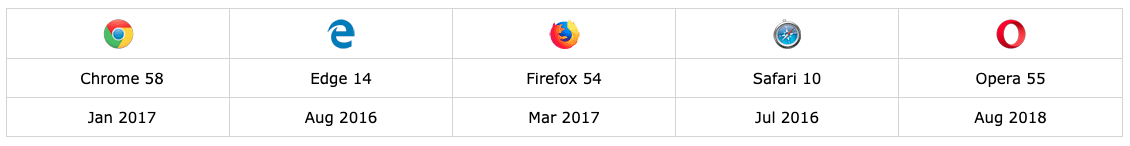
\includegraphics[scale=0.4]{./images/ES6_Support.png}
		 \caption{Supporto al linguaggio ECMAScript6. Immagine da: \url{https://www.w3schools.com/js/js_es6.asp}}
		 \label{SupportoECMAScript}	
	\end{center}
\end{figure}

\pagebreak

%\footnote{Il supporto al linguaggio ECMASCript 6 è il seguente:\\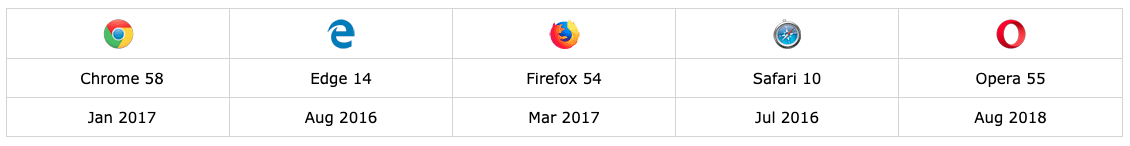
\includegraphics[scale=0.3]{./images/ES6_Support.png}\\Immagine da: \url{https://www.w3schools.com/js/js_es6.asp}} 

\subsection{Tacciamento Fonti-Requisiti}\label{Tracciamento}
\begin{center}
\begin{longtable}[c]{|c|m{.15\textwidth}|}
\hline
\rowcolor{bluelogo}\textbf{\textcolor{white}{Fonte}} & \textbf{\textcolor{white}{Requisiti}}\\
\hline \hline
\endhead
Capitolato & \makecell{ROQ1\\ROQ2\\RDQ5\\ROV4\\ROV6}\\
\hline
\rowcolor{grigio}Decisione Interna & \makecell{ROQ1.1\\RDQ1.2\\ROQ2.1\\RDQ2.2\\ROQ3\\RDQ6\\RDF1.6}\\
\hline
Piattaforma \textit{Grafana} & \makecell{ROV1\\ROV2\\ROV3\\ROV6}\\
\hline
\rowcolor{grigio}UC1 & \makecell{ROF1\\ROF1.1\\ROF1.2\\ROF1.3\\ROF1.4\\ROF1.4.1\\RFF1.4.2\\ROF1.5}\\
\hline
UC2 & \makecell{ROF2\\ROF2.1\\ROF2.1.1\\ROF2.1.2\\ROF2.5\\ROF2.5.10\\ROF2.6\\ROF2.7\\ROF2.8\\ROF2.8.1\\ROF2.8.3}\\
\hline
\rowcolor{grigio}UC2.2 & \makecell{ROF2.5.1\\ROF2.5.2\\ROF2.5.3\\ROF2.5.4\\ROF2.5.6\\ROF2.5.6.1\\ROF2.5.6.2\\RDF2.5.6.3\\ROF2.5.7\\ROF2.5.8\\ROF2.5.9}\\
\hline
UC3 & \makecell{ROF3\\ROF3.3\\ROF3.3.3\\ROF3.4\\ROF3.5}\\
\hline
\rowcolor{grigio}UC3.2 & \makecell{ROF3.3.1\\ROF3.3.2\\ROF3.3.2.1\\ROF3.3.2.2}\\
\hline
\rowcolor{grigio}UC4 & \makecell{ROF2.8.3\\ROF4\\ROF4.4\\ROF4.4.1\\ROF4.4.2\\ROF4.4.3\\ROF4.5\\ROF4.6\\RDF4.6.1}\\
\hline
UC5 & \makecell{RFF5\\RFF5.1\\RFF5.1.1\\RFF5.1.2}\\
\hline
\rowcolor{grigio}UC6 & \makecell{RFF6.2\\RFF6.2.1}\\
\hline
UC7 & \makecell{ROF2.8.3\\RFF6\\RFF6.1}\\
\hline
\rowcolor{grigio}UC8 & \makecell{ROF1.4\\ROF1.4.1\\RFF1.4.2}\\
\hline
UC9 & \makecell{ROF2.7}\\
\hline
\rowcolor{grigio}UC10 & \makecell{ROF4.5.1}\\
\hline
UC11 & \makecell{ROF4.5.2}\\
\hline
\rowcolor{grigio}UC12 & \makecell{ROF4.5.3}\\
\hline
UC13 & \makecell{ROF2.8\\ROF2.8.1\\ROF2.8.2\\ROF2.8.3}\\
\hline
\rowcolor{grigio}UC14 & \makecell{ROF2.5.9}\\
\hline
UC15 & \makecell{ROF3.5}\\
\hline
\rowcolor{grigio}VER-2019-02-08 & \makecell{RDF4.6.1\\RDF2.5.6.3}\\
\hline
Supporto a \textit{ECMAScript6} & \makecell{ROV8\\ROV9\\ROV10\\ROV11}\\
\hline
\caption{Tracciamento Fonti-Requisiti}
\end{longtable}
\end{center}


\subsection{Riepilogo Requisiti}\label{Riepilogo}
\begin{center}
\begin{longtable}[c]{|c|c|c|c|c|}
\hline
\rowcolor{bluelogo}\textbf{\textcolor{white}{Tipologia}} & \textbf{\textcolor{white}{Obbligatorio}} & \textbf{\textcolor{white}{Opzionale}} & \textbf{\textcolor{white}{Desiderabile}} & \textbf{\textcolor{white}{Totale}}\\
\hline \hline
\endhead
Funzionale & 44 & 11 & 2 & 57\\
\hline
\rowcolor{grigio}Di Qualità & 5 & 0 & 4 & 9\\
\hline
Di Vincolo & 12 & 0 & 0 & 12\\
\hline
\caption{Riepilogo dei Requisiti}
\end{longtable}
\end{center}